\PassOptionsToPackage{unicode=true}{hyperref} % options for packages loaded elsewhere
\PassOptionsToPackage{hyphens}{url}
\documentclass[ignorenonframetext,]{beamer}
\IfFileExists{pgfpages.sty}{\usepackage{pgfpages}}{}
\setbeamertemplate{caption}[numbered]
\setbeamertemplate{caption label separator}{: }
\setbeamercolor{caption name}{fg=normal text.fg}
\beamertemplatenavigationsymbolsempty
\usepackage{lmodern}
\usepackage{amssymb,amsmath}
\usepackage{ifxetex,ifluatex}
\usepackage{fixltx2e} % provides \textsubscript
\ifnum 0\ifxetex 1\fi\ifluatex 1\fi=0 % if pdftex
  \usepackage[T1]{fontenc}
  \usepackage[utf8]{inputenc}
\else % if luatex or xelatex
  \ifxetex
    \usepackage{mathspec}
  \else
    \usepackage{fontspec}
\fi
\defaultfontfeatures{Ligatures=TeX,Scale=MatchLowercase}







\fi

  \usetheme[]{metropolis}






% use upquote if available, for straight quotes in verbatim environments
\IfFileExists{upquote.sty}{\usepackage{upquote}}{}
% use microtype if available
\IfFileExists{microtype.sty}{%
  \usepackage{microtype}
  \UseMicrotypeSet[protrusion]{basicmath} % disable protrusion for tt fonts
}{}


\newif\ifbibliography


\hypersetup{
      pdftitle={Entrega},
        pdfauthor={Luiz Fernando Palin Droubi},
          pdfborder={0 0 0},
    breaklinks=true}
%\urlstyle{same}  % Use monospace font for urls




  \usepackage{color}
  \usepackage{fancyvrb}
  \newcommand{\VerbBar}{|}
  \newcommand{\VERB}{\Verb[commandchars=\\\{\}]}
  \DefineVerbatimEnvironment{Highlighting}{Verbatim}{commandchars=\\\{\}}
  % Add ',fontsize=\small' for more characters per line
  \usepackage{framed}
  \definecolor{shadecolor}{RGB}{248,248,248}
  \newenvironment{Shaded}{\begin{snugshade}}{\end{snugshade}}
  \newcommand{\AlertTok}[1]{\textcolor[rgb]{0.94,0.16,0.16}{#1}}
  \newcommand{\AnnotationTok}[1]{\textcolor[rgb]{0.56,0.35,0.01}{\textbf{\textit{#1}}}}
  \newcommand{\AttributeTok}[1]{\textcolor[rgb]{0.77,0.63,0.00}{#1}}
  \newcommand{\BaseNTok}[1]{\textcolor[rgb]{0.00,0.00,0.81}{#1}}
  \newcommand{\BuiltInTok}[1]{#1}
  \newcommand{\CharTok}[1]{\textcolor[rgb]{0.31,0.60,0.02}{#1}}
  \newcommand{\CommentTok}[1]{\textcolor[rgb]{0.56,0.35,0.01}{\textit{#1}}}
  \newcommand{\CommentVarTok}[1]{\textcolor[rgb]{0.56,0.35,0.01}{\textbf{\textit{#1}}}}
  \newcommand{\ConstantTok}[1]{\textcolor[rgb]{0.00,0.00,0.00}{#1}}
  \newcommand{\ControlFlowTok}[1]{\textcolor[rgb]{0.13,0.29,0.53}{\textbf{#1}}}
  \newcommand{\DataTypeTok}[1]{\textcolor[rgb]{0.13,0.29,0.53}{#1}}
  \newcommand{\DecValTok}[1]{\textcolor[rgb]{0.00,0.00,0.81}{#1}}
  \newcommand{\DocumentationTok}[1]{\textcolor[rgb]{0.56,0.35,0.01}{\textbf{\textit{#1}}}}
  \newcommand{\ErrorTok}[1]{\textcolor[rgb]{0.64,0.00,0.00}{\textbf{#1}}}
  \newcommand{\ExtensionTok}[1]{#1}
  \newcommand{\FloatTok}[1]{\textcolor[rgb]{0.00,0.00,0.81}{#1}}
  \newcommand{\FunctionTok}[1]{\textcolor[rgb]{0.00,0.00,0.00}{#1}}
  \newcommand{\ImportTok}[1]{#1}
  \newcommand{\InformationTok}[1]{\textcolor[rgb]{0.56,0.35,0.01}{\textbf{\textit{#1}}}}
  \newcommand{\KeywordTok}[1]{\textcolor[rgb]{0.13,0.29,0.53}{\textbf{#1}}}
  \newcommand{\NormalTok}[1]{#1}
  \newcommand{\OperatorTok}[1]{\textcolor[rgb]{0.81,0.36,0.00}{\textbf{#1}}}
  \newcommand{\OtherTok}[1]{\textcolor[rgb]{0.56,0.35,0.01}{#1}}
  \newcommand{\PreprocessorTok}[1]{\textcolor[rgb]{0.56,0.35,0.01}{\textit{#1}}}
  \newcommand{\RegionMarkerTok}[1]{#1}
  \newcommand{\SpecialCharTok}[1]{\textcolor[rgb]{0.00,0.00,0.00}{#1}}
  \newcommand{\SpecialStringTok}[1]{\textcolor[rgb]{0.31,0.60,0.02}{#1}}
  \newcommand{\StringTok}[1]{\textcolor[rgb]{0.31,0.60,0.02}{#1}}
  \newcommand{\VariableTok}[1]{\textcolor[rgb]{0.00,0.00,0.00}{#1}}
  \newcommand{\VerbatimStringTok}[1]{\textcolor[rgb]{0.31,0.60,0.02}{#1}}
  \newcommand{\WarningTok}[1]{\textcolor[rgb]{0.56,0.35,0.01}{\textbf{\textit{#1}}}}



% Prevent slide breaks in the middle of a paragraph:
\widowpenalties 1 10000
\raggedbottom

  \AtBeginPart{
    \let\insertpartnumber\relax
    \let\partname\relax
    \frame{\partpage}
  }
  \AtBeginSection{
    \ifbibliography
    \else
      \let\insertsectionnumber\relax
      \let\sectionname\relax
      \frame{\sectionpage}
    \fi
  }
  \AtBeginSubsection{
    \let\insertsubsectionnumber\relax
    \let\subsectionname\relax
    \frame{\subsectionpage}
  }



\setlength{\parindent}{0pt}
\setlength{\parskip}{6pt plus 2pt minus 1pt}
\setlength{\emergencystretch}{3em}  % prevent overfull lines
\providecommand{\tightlist}{%
  \setlength{\itemsep}{0pt}\setlength{\parskip}{0pt}}

  \setcounter{secnumdepth}{0}


  \usepackage[brazil]{babel} \usepackage{booktabs}

  \title[]{Entrega}

  \subtitle{Secretaria de Pesca e Aquicultura\\
10154.129510/2020-10}

  \author[
        Luiz Fernando Palin Droubi
    ]{Luiz Fernando Palin Droubi}

  \institute[
    ]{
    Superintendência do Patrimônio da União em Santa Catarina - SPU/SC
    }

\date[
      2020-10-16
  ]{
      2020-10-16
        }


\begin{document}

% Hide progress bar and footline on titlepage
  \begin{frame}[plain]
  \titlepage
  \end{frame}



\begin{frame}{IMAGEM DOS POLÍGONOS ENVIADOS}
\protect\hypertarget{imagem-dos-poluxedgonos-enviados}{}

\begin{center}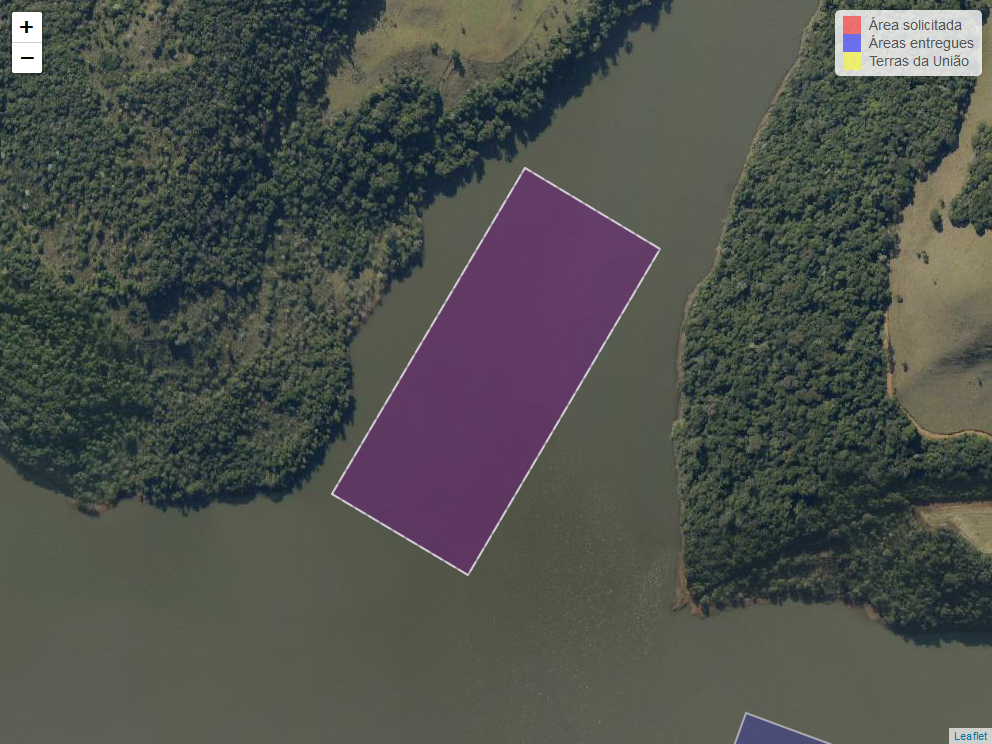
\includegraphics[width=1\linewidth]{imagem_10154-129510-2020-10} \end{center}

\end{frame}

\begin{frame}{Tabela de coordenadas}
\protect\hypertarget{tabela-de-coordenadas}{}

\begin{table}[H]
\centering\begingroup\fontsize{6}{8}\selectfont

\begin{tabular}{lrrrrr}
\toprule
\multicolumn{1}{c}{Vértice} & \multicolumn{2}{c}{Coordenadas} & \multicolumn{2}{c}{Azimutes} & \multicolumn{1}{c}{Distância} \\
\cmidrule(l{3pt}r{3pt}){1-1} \cmidrule(l{3pt}r{3pt}){2-3} \cmidrule(l{3pt}r{3pt}){4-5} \cmidrule(l{3pt}r{3pt}){6-6}
  & E & N & Real & Plano & (m)\\
\midrule
VT1 & 425.324,458 & 6.960.663,051 & 30,74848 & 31,81125 & 399,9289\\
VT2 & 425.526,834 & 6.961.007,996 & 120,74525 & 121,80802 & 167,3333\\
VT3 & 425.671,165 & 6.960.923,326 & 210,71372 & 211,77649 & 399,7875\\
VT4 & 425.469,060 & 6.960.578,386 & 300,69721 & 301,75998 & 167,5646\\
VT1.1 & 425.324,458 & 6.960.663,051 & NA & NA & NA\\
\bottomrule
\end{tabular}
\endgroup{}
\end{table}

\end{frame}

\begin{frame}{Memorial}
\protect\hypertarget{memorial}{}

\tiny Inicia-se este memorial pelo vértice \textbf{VT1} com coordenadas
\textbf{N 6.960.663,05} e \textbf{E 425.324,46}. Deste segue com azimute
31,81° e distância 399,93m até o vértice \textbf{VT2} com coordenadas
\textbf{N 6.961.008,00} e \textbf{E 425.526,83}. Deste segue com azimute
121,81° e distância 167,33m até o vértice \textbf{VT3} com coordenadas
\textbf{N 6.960.923,33} e \textbf{E 425.671,16}. Deste segue com azimute
211,78° e distância 399,79m até o vértice \textbf{VT4} com coordenadas
\textbf{N 6.960.578,39} e \textbf{E 425.469,06}. Deste segue com azimute
301,76° e distância 167,56m até o vértice \textbf{VT1}, origem desta
descrição.

\end{frame}

\begin{frame}{Atributos}
\protect\hypertarget{atributos}{}

\begin{table}[H]
\centering\begingroup\fontsize{8}{10}\selectfont

\begin{tabular}{ll}
\toprule
  & 1\\
\midrule
destinacao & entrega\\
tipo & aquatica\\
rip & NA\\
interessado & Quality Fish Brasil Ltda EPP\\
area & 66955.83 [m\textasciicircum{}2]\\
\addlinespace
area\_uniao & 66955.83 [m\textasciicircum{}2]\\
nup & 10154.129510/2020-10\\
protocolo & Ofício MAPA - 8973358 (7494143)\\
ref & 8415439\\
municipio & 8257\\
\addlinespace
logradouro & NA\\
trecho & NA\\
aval & 1053.79\\
dataaval & 2019-09-09\\
\bottomrule
\end{tabular}
\endgroup{}
\end{table}

\end{frame}

\begin{frame}[fragile]{Salvar no disco}
\protect\hypertarget{salvar-no-disco}{}

\scriptsize

\begin{Shaded}
\begin{Highlighting}[]
\KeywordTok{st_write}\NormalTok{(spl_df, }\KeywordTok{paste}\NormalTok{(nup, }\StringTok{".geojson"}\NormalTok{, }\DataTypeTok{sep =} \StringTok{""}\NormalTok{), }
         \DataTypeTok{delete_dsn =} \OtherTok{TRUE}\NormalTok{)}
\end{Highlighting}
\end{Shaded}

\begin{verbatim}
## Deleting source `10154-129510-2020-10.geojson' failed
## Writing layer `10154-129510-2020-10' to data source `10154-129510-2020-10.geojson' using driver `GeoJSON'
## Writing 1 features with 14 fields and geometry type Polygon.
\end{verbatim}

\end{frame}




\end{document}
